\documentclass{article}

%math package
\usepackage{amsmath}
\usepackage{amsthm}
\usepackage{amsfonts}
\usepackage{amssymb}
%document package
\usepackage[utf8]{vietnam}
\usepackage{titlesec}
\usepackage{listings}
\usepackage{graphicx}
\usepackage[document]{ragged2e}
\usepackage{caption}
\usepackage{soul}
\usepackage{float}
\usepackage{subfigure}
\usepackage{multicol}
\usepackage{multirow}
\usepackage{longtable}
\usepackage{geometry}
\geometry{legalpaper, portrait, margin=1in}

%setup environment
\setcounter{secnumdepth}{4}
\graphicspath{{images/}}
%
\captionsetup{belowskip=12pt,aboveskip=4pt}
\begin{document}
	
%--------------------------title page-------------------------------------
\thispagestyle{empty}
\begin{titlepage}
\begin{center}
	\textbf{\huge{Khai thác dữ liệu và ứng dụng}}\\
	\Large{BT01: Khai thác tập phổ biến \& Luật kết hợp}	
\end{center}	

\vfill
\begin{flushright}
	\begin{tabular}{l l l}
		GVLT: & \quad Thầy Lê Hoài Bắc\\
		GVTH: & \quad Thầy Nguyễn Tiến Huy\\
		Sinh viên: & \quad Nguyễn Phan Mạnh Hùng & 1312727\\
		& \quad La Ngọc Thùy An & 1312716\\
	\end{tabular}
\end{flushright}
\end{titlepage}
\pagebreak
%-------------------------Mục lục-----------------------------------------
\thispagestyle{empty}
\tableofcontents
\pagebreak 
%-------------------------Bài 1------------------------------------------- 
\pagenumbering{arabic}
\section{Bài 1: Apriori}\label{sec: prob1}
\subsection{Câu 1}
\subsubsection{Tập phổ biến}
\begin{table}[H]
\begin{tabular}[t]{|c | c | c | c|}
	\hline
	Kích thước & ID & Tập phổ biến  & Support \\ \hline
	\multirow{7}{*}{1} & 1 & Bread & 4 \\
	&2& Peanuts & 4 \\
	&3& Milk & 6 \\
	&4& Fruit & 6 \\
	&5& Jam & 5 \\
	&6& Soda & 6 \\
	&7& Chips & 4 \\ 
	\hline
	\multirow{10}{*}{2}&8& Bread Milk& 3\\
	&9& Bread Jam& 4\\
	&10& Bread Soda& 3\\
	&11& Bread Chips& 3\\
	&12& Peanuts Milk& 3\\
	&13& Peanuts Fruit& 4\\
	&14& Milk Fruit& 5\\
	&15& Milk Jam& 4\\
	&16& Milk Soda& 5\\
	&17& Milk Chips & 3\\

	\hline
\end{tabular}~%
\begin{tabular}[t]{|c | c | c | c|}
	\hline
	Kích thước & ID & Tập phổ biến  & Support \\ \hline
	\multirow{5}{*}{2}&18& Fruit Jam& 3\\
	&19&Fruit Soda& 4\\
	&20&Jam Soda& 4\\
	&21& Jam Chips& 3\\
	&22& Soda Chips& 4\\
	\hline 
	\multirow{15}{*}{3}&23&Bread Milk Jam& 3\\
	&24&Bread Jam Soda& 3\\
	&25&Bread Jam Chips& 3\\
	&26&Bread Soda Chips& 3\\
	&27&Peanuts Milk Fruit& 3\\
	&28&Milk Fruit Jam& 3\\
	&29&Milk Fruit Soda& 4\\
	&30&Milk Jam Soda& 3\\
	&31&Milk Soda Chips& 3\\
	&32&Jam Soda Chips& 3\\
	\hline
	4&33&Bread Jam Soda Chips& 3\\
	\hline
\end{tabular}
\end{table}
\subsubsection{Thiết lập tham số - Tập phổ biến sinh bởi Weka}
\begin{figure}[H]
	\centering
	\caption{Màn hình thiết lập tham số}
	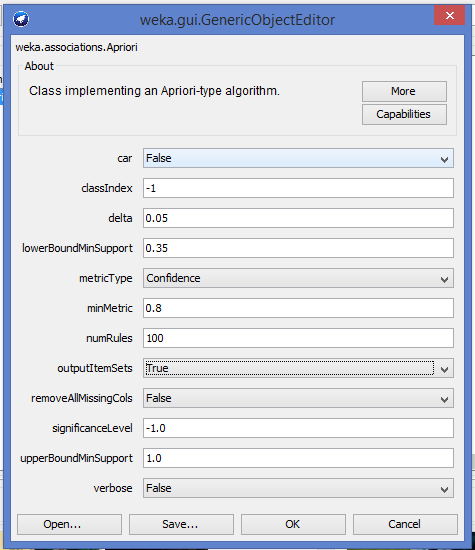
\includegraphics[scale = 0.5]{para}
	
\end{figure}
\begin{figure}[H]
	\centering
	\caption{Màn hình kết quả tập phổ biến}
	\begin{minipage}{0.4\textwidth}
		\centering
		\includegraphics[scale = 0.5]{freset1}
	\end{minipage}%
	\begin{minipage}{0.4\textwidth}
		\centering
		\includegraphics[scale = 0.5]{freset2}
	\end{minipage}%
	\begin{minipage}{0.4\textwidth}
		\centering
		\includegraphics[scale = 0.5]{freset3}
	\end{minipage}%
\end{figure}

\subsection{Câu 2}
%\begin{tabular}
%\end{tabular}
\subsubsection{Luật kết hợp}
\begin{table}[H]
\begin{longtable}{|c | c | c  c  c | c|}
	
	\hline
    Rule ID & Set ID & Rule &&& Confidence\\
    \hline
	1 & \multirow{2}{*}{8}&Bread 4 & $\to$ & Jam 4& 1\\ 
	2 & &Jam 5 & $\to$ & Bread 4& 0.8\\ \hline	
	3 & 13&Peanuts 4 & $\to$ & Fruit 4& 1\\ \hline	
	4 & 22&Chips 4 & $\to$ & Soda 4& 1\\ \hline	
	5 & \multirow{2}{*}{14}&Fruit 6 & $\to$ & Milk 5& 0.83\\
	6 & &Milk 6 & $\to$ & Fruit 5& 0.83\\ \hline	
	7 & \multirow{2}{*}{16}&Soda 6 & $\to$ & Milk 5& 0.83\\
	8 & &Milk 6 & $\to$ & Soda 5& 0.83\\ \hline	
	9 & 15&Jam 5 & $\to$ & Milk 4& 0.8\\ \hline	
	10& 20&Jam 5 & $\to$ & Soda 4& 0.8\\ \hline	
	11& 19&Fruit Soda 4 & $\to$ & Milk 4& 1\\ \hline	
	12& 23&Bread Milk 3 & $\to$ & Jam 3& 1\\ \hline	
	13& 24&Bread Soda 3 & $\to$ & Jam 3& 1\\ \hline	
	14& \multirow{2}{*}{25}&Jam Chips 3 & $\to$ & Bread 3& 1\\
	15& &Bread Chips 3 & $\to$ & Jam 3& 1\\	\hline
	16& \multirow{2}{*}{26}&Bread Chips 3 & $\to$ & Soda 3& 1\\
	17& &Bread Soda 3 & $\to$ & Chips 3& 1\\ \hline	
	18& 27&Peanuts Milk 3 & $\to$ & Fruit 3& 1\\ \hline
	19& 28&Fruit Jam 3 & $\to$ & Milk 3& 1\\ \hline	
	20& 31&Milk Chips 3 & $\to$ & Soda 3& 1\\ \hline	
	21& 32&Jam Chips 3 & $\to$ & Soda 3& 1\\ \hline	
	22& \multirow{2}{*}{29}&Milk Soda 5 & $\to$ & Fruit 4& 0.8\\
	23& &Milk Fruit 5 & $\to$ & Soda 4& 0.8\\ \hline	
	24& \multirow{7}{*}{33}&Jam Soda Chips 3 & $\to$ & Bread 3& 1\\
	25& &Bread Soda Chips 3 & $\to$ & Jam 3& 1\\
	26& &Bread Jam Chips 3 & $\to$ & Soda 3& 1\\
	27& &Bread Jam Soda 3 & $\to$ & Chips 3& 1\\
	28& &Jam Chips 3 & $\to$ & Bread Soda 3& 1\\
	29& &Bread Chips 3 & $\to$ & Jam Soda 3& 1\\
	30& &Bread Soda 3 & $\to$ & Jam Chips 3& 1\\
	\hline
\end{longtable}
\end{table}
\subsubsection{Kết quả luật kết hợp}
\begin{figure}[H]
	\centering
	\caption{Kết quả luật kết hợp bằng Weka}
	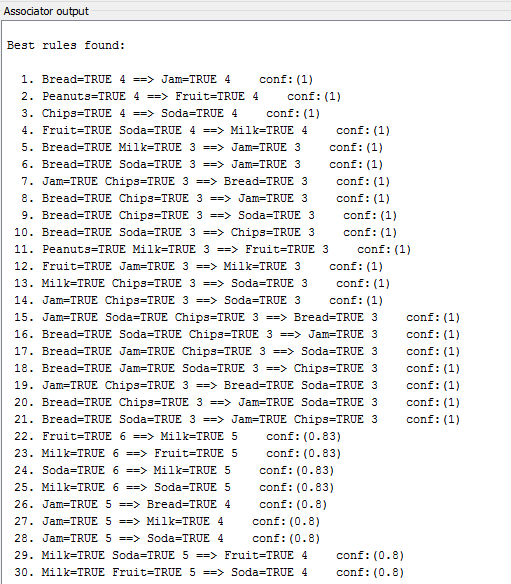
\includegraphics[scale = 0.7]{Rule}
\end{figure}
%\pagebreak
%-------------------------Bài 2------------------------------------------- 
\section{Bài 2: FP-Growth}\label{sec: prob2}
\subsection{Câu 1}
\begin{flushleft}
Bước 1: Duyệt cơ sở dữ liệu, chọn ra các item phổ biến và sắp xếp giảm dần. Ta được:\\
\begin{center}
\begin{tabular}{|c|c|c|c|c|c|c|}
	\hline Milk & Fruit & Soda & Jam & Chips & Peanuts & Bread \\ 
	\hline 6 & 6 & 6 & 5 & 4 & 4 & 4 \\ 
	\hline 
\end{tabular} 
\end{center}
Bước 2: Duyệt cơ sở dữ liệu lần hai. Với mỗi transaction, ta sắp xếp các item theo thứ tự độ phổ biến giảm dần trong bảng trên. Ta được:\\
\begin{center}
\begin{tabular}{c|c c c c c c }
	Tid & \multicolumn{6}{c}{Items}  \\ 
	\hline 1 & Milk & Fuit & Jam & Peanuts & Bread &  \\ 
	2 & Milk & Fruit & Soda & Jam & Chips & Bread \\ 
	3 & Soda & Jam & Chips & Bread &  &  \\ 
	4 & Milk & Fruit & Soda & Jam & Peanuts &  \\ 
	5 & Milk & Soda & Jam & Chips & Bread &  \\ 
	6 & Milk & Fruit & Soda & Chips &  &  \\ 
	7 & Milk & Fruit & Soda & Peanuts &  &  \\ 
	8 & Fruit & Peanuts &  &  &  &  \\ 
\end{tabular} 
\end{center}



Bước 3: Xây dựng cây FP-growth\\ 
\begin{center}
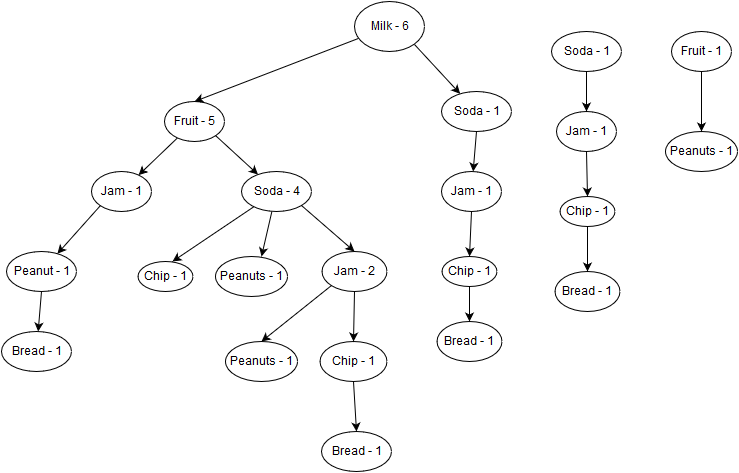
\includegraphics[scale = 0.5]{Tree.png}
\end{center}
Bước 4: Xây dựng các cơ sở dữ liệu điều kiện và sắp xếp theo thứ tự giảm dần của support, đồng thời loại bỏ các item không thỏa min support.
\begin{table}[H]
	\centering	
	\caption{CSDL điều kiện - Bread}
	\begin{tabular}{|c | c | c | c | c | c |}
		\hline
		Bread & & & & &\\ \hline
		& Jam - 1 & Milk - 1 & \st{Peanuts} & \st{Fruit} & \\ \hline
		& Jam - 1 & Milk - 1 & Chips - 1 & Soda - 1 & \st{Fruit}\\ \hline
		& Jam - 1 & Milk - 1 & Chips - 1 & Soda - 1 & \\ \hline
		& Jam - 1 & Chips - 1 & Soda - 1 & & \\ \hline
	\end{tabular}
\end{table}
\begin{table}[H]
	\begin{minipage}[t]{0.5\linewidth}
		\centering
		\caption{CSDL điều kiện - Peanuts}
		\begin{tabular}{| c | c | c | c | c |}
			\hline
			Peanuts &&&& \\ \hline
			& Fruit - 1 & Milk - 1 & \st{Jam} & \\ \hline
			& Fruit - 1 & Milk - 1 & \st{Soda} & \\ \hline
			& Fruit - 1 & Milk - 1 & \st{Soda} & \st{Jam} \\ \hline
			& Fruit - 1 &&& \\ \hline
		\end{tabular}
	\end{minipage}%
	\begin{minipage}[t]{0.5\linewidth}
		\centering
		\caption{CSDL điều kiện - Chips}
		\begin{tabular}{| c | c | c | c | c |}
			\hline
			Chips &&&& \\ \hline
			&Soda - 1 & Milk - 1 & \st{Fruit} &\\ \hline
			&Soda - 1 & Milk - 1 & Jam - 1 & \st{Fruit} \\ \hline
			&Soda - 1 & Milk - 1 & Jam - 1 & \\ \hline
			&Soda - 1 & Jam - 1 && \\ \hline
		\end{tabular}
	\end{minipage}
\end{table}
\begin{table}[H]
	\begin{minipage}[t]{0.4\linewidth}
		\centering
		\caption{CSDL điều kiện - Jam}
		\begin{tabular}{| c | c | c | c |}
			\hline
			Jam &&& \\ \hline
			&Milk - 1 & Fruit - 1 & \\ \hline
			&Milk - 2 & Soda - 2 & Fruit - 2  \\ \hline
			&Milk - 1 & Soda - 1 &  \\ \hline
			&Soda - 1 & & \\ \hline
		\end{tabular}
	\end{minipage}%
	\begin{minipage}[t]{0.35\linewidth}
		\centering
		\caption{CSDL điều kiện - Soda}
		\begin{tabular}{| c | c | c |}
			\hline
			Soda && \\ \hline
			&Milk - 4 & Fruit - 4  \\ \hline
			&Milk - 1 &  \\ \hline
		\end{tabular}
	\end{minipage}%
	\begin{minipage}[t]{0.3\linewidth}
		\centering
		\caption{CSDL điều kiện - Fruit}
		\begin{tabular}{| c | c |}
			\hline
			Fruit & \\ \hline
			&Milk - 5   \\ \hline
		\end{tabular}
	\end{minipage}%

\end{table}
Ở đây ta được các tập phổ biến (ứng với mỗi điều kiện):\\
\begin{multicols}{3}
\begin{itemize}
	\item Bread
	\item Peanuts
	\item Chips
	\item Jam
	\item Soda
	\item Fruit
	\item Milk
\end{itemize}
\end{multicols}
Bước 5: Xây dựng các FP-trees tương ứng:
\begin{figure}[H]
	\centering
	\begin{minipage}[t]{0.5\textwidth}
		\centering
		\caption{Bread - FP tree}
		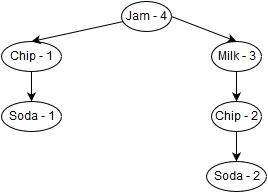
\includegraphics[scale = 0.5]{BreadTree}
	\end{minipage}%
	\begin{minipage}[t]{0.5\textwidth}
		\centering
		\caption{Peanuts - FP tree}
		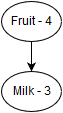
\includegraphics[scale = 0.5]{PeanutsTree}
	\end{minipage}
\end{figure}
\begin{figure}[H]
	\centering
	\begin{minipage}[t]{0.5\textwidth}
		\centering
		\caption{Chips - FP tree}
		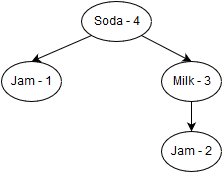
\includegraphics[scale = 0.5]{ChipsTree}
	\end{minipage}%
	\begin{minipage}[t]{0.5\textwidth}
		\centering
		\caption{Jam - FP tree}
		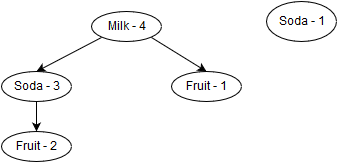
\includegraphics[scale = 0.5]{JamTree}
	\end{minipage}
\end{figure}
\begin{figure}[H]
	\centering
	\begin{minipage}[t]{0.5\textwidth}
		\centering
		\caption{Soda - FP tree}
		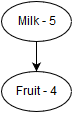
\includegraphics[scale = 0.5]{SodaTree}
	\end{minipage}%
	\begin{minipage}[t]{0.5\textwidth}
		\centering
		\caption{Fruit - FP tree}
		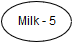
\includegraphics[scale = 0.5]{FruitTree}
	\end{minipage}
\end{figure}



Ta thấy các cây điều kiện Peanuts, Soda, và Fruit suy biến, nên ta tiến hành khai thác các tập phổ biến:
\begin{multicols}{3}
\begin{itemize}
	\item Peanuts Fruit
	\item Peanuts Milk
	\item Peanuts Fruit Milk
	\item Soda Fruit
	\item Soda Milk
	\item Soda Fruit Milk
	\item Fruit Milk
\end{itemize}
\end{multicols}
Sau đó ta lại tiếp tục đệ quy xây dựng các cơ sở dữ liệu điều kiện và cây FP cho tới khi các cây suy biến để khai thác tập phổ biến.\\
Cụ thể:\\
\begin{center}
\begin{tabular}{|c|c|c|c|}
	\hline
	Điều kiện & Transactions & FP-tree & Tập phổ biến \\ 
	\hline
	Bread Soda & Chips - 1, Jam - 1 & (Chips - 3 $\to$ Jam - 3) & Bread Soda \\ 
	& Chips - 2, Jam - 2, \st{Milk} &  & Bread Soda Chips \\ 
	&  &  &  Bread Soda Jam\\
	&  &  &  Bread Soda Chips Jam\\ 
	\hline
	Bread Chips & Jam 1 & (Jam - 3) &Bread Chips\\
	& Jam - 2, \st{Milk} &  & Bread Chips Jam\\
	\hline
	Bread Milk & Jam - 3 & (Jam - 3)& Bread Milk\\
	&  &  &  Bread Milk Jam\\
	\hline
	Bread Jam & $\varnothing$ & $\varnothing$ &Bread Jam\\   
	\hline
	Chips Jam & Soda - 1 & (Soda - 3) & Chips Jam\\
	& Soda - 2, \st{Milk} &  & Chips Jam Soda\\
	\hline
	Chips Milk & Soda - 3 & (Soda - 3) & Chips Milk\\
	&  &  & Chips Milk Soda\\
	\hline
	Chips Soda & $\varnothing$ & $\varnothing$ & Chips Soda\\
	\hline
	Jam Fruit & Milk - 2, \st{Soda} & (Milk-3) & Jam Fruit\\
	& Milk - 1 &  & Jam Fruit Milk\\
	\hline
	Jam Soda & Milk - 3 & (Milk - 3) & Jam Soda \\
	&  &  & Jam Soda Milk\\
	\hline 
	Jam Milk & $\varnothing$ & $\varnothing$ & Jam Milk\\
	\hline
\end{tabular} 
\end{center}
\subsection{Câu 2}
Các tập phổ biến được sinh ra bởi thuật toán Apriori theo thứ tự kích thước từ nhỏ tới lớn. Trong khi đó, nếu dùng FP-growth thì các tập kích thước lớn có thể được sinh ra trước.\\
Tuy vậy, các tập phổ biến được sinh ra bởi 2 thuật là giống nhau.
\end{flushleft}

%\pagebreak
%-------------------------Bài 3------------------------------------------- 


\section{Bài 3: Các độ đo lý thú}\label{sec: prob3}
\subsection{Câu 1}
\begin{flushleft}
	\underline{Quy ước:}
	\begin{tabular}{l l}
		B, C: &  itemset\\
		$conf\left(B \to C\right)$: &  độ đo \textbf{confidence} của luật $B \to C$ \\
		$lift\left(B, C\right):$ &  độ đo \textbf{lift} của luật $B \to C$ và C $\to B$ (do có cách tính tương tự)\\
		$conv\left(B \to C\right):$ &  độ đo \textbf{conviction} của luật $B \to C$ \\ 
		$leve\left(B \to C\right):$ &  độ đo \textbf{leverage} của luật $B \to C$ \\
	\end{tabular}
\end{flushleft}
\subsubsection{Confidence}
\begin{equation}
	conf\left(B \to C \right) = \frac{sup \left( B \cup C \right)}{sup \left( B\right)}
\end{equation}
Ý nghĩa: thể hiện tỉ lệ các transaction chứa itemset B thì chứa cả itemset C, hay có thể hiểu như tỉ lệ luật dự đoán chính xác.
\subsubsection{Lift}
\begin{equation}
	lift\left( B,C \right) = \frac{conf\left( B \to C \right)}{sup \left( C \right)} = \frac{sup \left(B \cup C \right)}{sup \left( B\right) \times sup \left( C \right)}
\end{equation}
Ý nghĩa: Thể hiện sự độc lập giữa itemset B và itemset C. Nếu lift = 1, thì 2 itemsets này độc lập. Nếu lift < 1 thì nó thể hiện tính negative correlated, tức sự xuất hiện của itemset này ảnh hưởng ít tới sự xuất hiện của itemset kia. Nếu lift > 1 thì sự xuất hiện của itemset này ảnh hưởng nhiều tới sự xuất hiện của itemset kia, hay còn gọi là positive correlated.
\subsubsection{Conviction}
\begin{equation}
	conv\left( B \to C \right) = \frac{1 - sup \left( C \right)}{1 - conf \left( B \to C \right)}
\end{equation}
Ý nghĩa: thể hiện tỉ lệ itemset B xuất hiện mà không có C. Nói cách khác, thể hiện tần số luật B $\to$ C dự đoán sai.
\subsubsection{Leverage}
\begin{equation}
	leve(B \to C) = sup \left(B \cup C \right) - sup\left(B\right) \times sup\left(C\right)
\end{equation}

\subsection{Câu 2}
\begin{table}[H]
	\centering
	\begin{tabular}{|c | c c c c|}
		\hline
		Rule Id & Confidence & Lift & Leverage & Conviction\\ \hline 
	%	1 & 1.00 & 1.60 & 0.19 & 0.00 \\ 
	%	2 & 0.80 & 1.60 & 0.19 & 0.00 \\ 
	%	3 & 1.00 & 1.33 & 0.13 & 0.00 \\ 
	%	4 & 1.00 & 1.33 & 0.13 & 0.00 \\ 
	%	5 & 0.83 & 1.11 & 0.06 & 0.00 \\ 
	%	6 & 0.83 & 1.11 & 0.06 & 0.00 \\ 
	%	7 & 0.83 & 1.11 & 0.06 & 0.00 \\ 
	%	8 & 0.83 & 1.11 & 0.06 & 0.00 \\ 
	%	9 & 0.80 & 1.07 & 0.03 & 0.00 \\ 
	%	10 & 0.80 & 1.07 & 0.03 & 0.00 \\ 
	%	11 & 1.00 & 1.33 & 0.13 & 0.00 \\ 
	%	12 & 1.00 & 1.60 & 0.14 & 0.00 \\ 
	%	13 & 1.00 & 1.60 & 0.14 & 0.00 \\ 
	%	14 & 1.00 & 2.00 & 0.19 & 0.00 \\ 
	%	15 & 1.00 & 1.60 & 0.14 & 0.00 \\ 
		1 & 1.00 & 1.60 & 0.19 & $\infty$ \\ 
		2 & 0.80 & 1.60 & 0.19 & 2.50 \\ 
		3 & 1.00 & 1.33 & 0.13 & $\infty$ \\ 
		4 & 1.00 & 1.33 & 0.13 & $\infty$ \\ 
		5 & 0.83 & 1.11 & 0.06 & 1.50 \\ 
		6 & 0.83 & 1.11 & 0.06 & 1.50 \\ 
		7 & 0.83 & 1.11 & 0.06 & 1.50 \\ 
		8 & 0.83 & 1.11 & 0.06 & 1.50 \\ 
		9 & 0.80 & 1.07 & 0.03 & 1.25 \\ 
		10 & 0.80 & 1.07 & 0.03 & 1.25 \\ 
		11 & 1.00 & 1.33 & 0.13 & $\infty$ \\ 
		12 & 1.00 & 1.60 & 0.14 & $\infty$ \\ 
		13 & 1.00 & 1.60 & 0.14 & $\infty$ \\ 
		14 & 1.00 & 2.00 & 0.19 & $\infty$ \\ 
		15 & 1.00 & 1.60 & 0.14 & $\infty$ \\ 
		\hline
	\end{tabular}~%
	\begin{tabular}{|c | c c c c|}
		\hline
		Rule Id & Confidence & Lift & Leverage & Conviction\\ \hline 
	%	16 & 1.00 & 1.33 & 0.09 & 0.00 \\ 
	%	17 & 1.00 & 2.00 & 0.19 & 0.00 \\ 
	%	18 & 1.00 & 1.33 & 0.09 & 0.00 \\ 
	%	19 & 1.00 & 1.33 & 0.09 & 0.00 \\ 
	%	20 & 1.00 & 1.33 & 0.09 & 0.00 \\ 
	%	21 & 1.00 & 1.33 & 0.09 & 0.00 \\ 
	%	22 & 0.80 & 1.07 & 0.03 & 0.00 \\ 
	%	23 & 0.80 & 1.07 & 0.03 & 0.00 \\ 
	%	24 & 1.00 & 2.00 & 0.19 & 0.00 \\ 
	%	25 & 1.00 & 1.60 & 0.14 & 0.00 \\ 
	%	26 & 1.00 & 1.33 & 0.09 & 0.00 \\ 
	%	27 & 1.00 & 2.00 & 0.19 & 0.00 \\ 
	%	28 & 1.00 & 2.67 & 0.23 & 0.00 \\ 
	%	29 & 1.00 & 2.00 & 0.19 & 0.00 \\ 
	%	30 & 1.00 & 2.67 & 0.23 & 0.00 \\ 
		16 & 1.00 & 1.33 & 0.09 & $\infty$ \\ 
		17 & 1.00 & 2.00 & 0.19 & $\infty$ \\ 
		18 & 1.00 & 1.33 & 0.09 & $\infty$ \\ 
		19 & 1.00 & 1.33 & 0.09 & $\infty$ \\ 
		20 & 1.00 & 1.33 & 0.09 & $\infty$ \\ 
		21 & 1.00 & 1.33 & 0.09 & $\infty$ \\ 
		22 & 0.80 & 1.07 & 0.03 & 1.25 \\ 
		23 & 0.80 & 1.07 & 0.03 & 1.25 \\ 
		24 & 1.00 & 2.00 & 0.19 & $\infty$ \\ 
		25 & 1.00 & 1.60 & 0.14 & $\infty$ \\ 
		26 & 1.00 & 1.33 & 0.09 & $\infty$ \\ 
		27 & 1.00 & 2.00 & 0.19 & $\infty$ \\ 
		28 & 1.00 & 2.67 & 0.23 & $\infty$ \\ 
		29 & 1.00 & 2.00 & 0.19 & $\infty$ \\ 
		30 & 1.00 & 2.67 & 0.23 & $\infty$ \\ 
		\hline
	\end{tabular}
\end{table}
\subsection{Câu 3}
\begin{figure}[H]
	\centering
	\caption{Giá trị Confidence, Lift, Leverage, Conviction tính bằng Weka}
	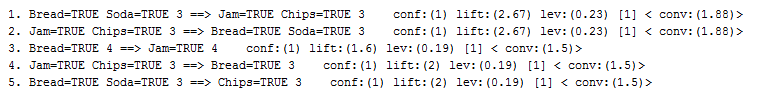
\includegraphics[scale = 0.8]{Measure}
\end{figure}
\subsection{Câu 4}
	Có sự khác biệt trong cách tính bằng công thức thông thường và trong Weka ở cột Conviction. Có thể chương trình đã thêm vào các hệ số làm trơn nhằm khử trường hợp không xác định khi $confidence = 1$ nhằm giữ được mối liên hệ giữa các itemset cho việc tính toán sau này.
\end{document}